\section{GUI}
\subsection{GUI Code}
\counterwithin{figure}{section}
\lstset{basicstyle=\tiny}
\begin{lstlisting}[language=Python,caption={GUI.py},label={lst:GUI.py}]
#Written by Brendon Camm, last updated March 27th, 2017

import sys
from PyQt5 import QtCore, QtGui, uic, QtWidgets
import matplotlib
from matplotlib.backends.backend_qt5agg import (FigureCanvasQTAgg as FigureCanvas,
NavigationToolbar2QT as NavigationToolBar)
from matplotlib.figure import Figure
import numpy as np
import time
import struct
import socket
from timeit import default_timer as timer
from PS4_Controller import PS4Controller as PS4
import threading
import logging
import matplotlib.animation as animation
import pyqtgraph as pg


qtCreatorFile = "GUI.ui" # Enter file here.
Ui_MainWindow, QtBaseClass = uic.loadUiType(qtCreatorFile)



class GUI(QtWidgets.QMainWindow, Ui_MainWindow, QtWidgets.QMenu):   
def __init__(self):

super(GUI,self).__init__()
#Qt initialization
QtWidgets.QMainWindow.__init__(self)
Ui_MainWindow.__init__(self)
self.page = QtWidgets.QStackedWidget()
self.setCentralWidget(self.page)
self.setupUi(self)
self.setWindowTitle("Drone")
self.setWindowIcon(QtGui.QIcon('smu.png'))

#Networking
self.getHost = socket.gethostname()
self.staticPort = '1247'
#Main Page buttons
self.start.clicked.connect(self.connection)
self.end.clicked.connect(self.stop)

#Listing widget
self.list.insertItem(0, 'Home')
self.list.insertItem(1, 'Controller')
self.list.currentRowChanged.connect(self.display)

#Controller Page
self.axisVal.setText('1 2 3 4')
self.hostVal.setText(self.getHost)
self.portVal.setText('2222')
self.axisMenu.clicked.connect(self.axisSettings)
self.hostMenu.clicked.connect(self.hostSettings)
self.portMenu.clicked.connect(self.portSettings)
self.updateConnect.clicked.connect(self.updateConnection)
self.connectPS4.clicked.connect(self.connectController)

#Live Plotting
self.initplt()
self.plotcurve = pg.PlotDataItem()
self.plotwidget.addItem(self.plotcurve)
self.t = 0
self.amplitude = 10
self.update1()
self.timer = pg.QtCore.QTimer()
self.timer.timeout.connect(self.move)
self.timer.start(1000)

def stop(self):
sys.exit(app.exec_())
def connection(self):
s = socket.socket()
host = self.getHost
port = int(self.staticPort)
status = s.connect_ex((host,port)) #Returns 0 if true
if status: # Status = errno
self.thisworks.setText("Connection Unsuccessful")
self.connectionStat.setText("Communications have not been established")
else: # Status = 0
print(status)
self.thisworks.setText("Connection Successful")
self.connectionStat.setText("Communications are active")
def axisSettings(self):
cont = PS4()
text, ok = QtWidgets.QInputDialog.getText(self, 'Axis Value[0]', 'No Spaces')
text1, ok = QtWidgets.QInputDialog.getText(self, 'Axis Value[1]', 'No Spaces')
text2, ok = QtWidgets.QInputDialog.getText(self, 'Axis Value[2]', 'No Spaces')
text3, ok = QtWidgets.QInputDialog.getText(self, 'Axis Value[3]', 'No Spaces')
axis = [int(text), int(text1), int(text2), int(text3)]
self.axisVal.setText(str(axis))
cont.axis_order = axis
return cont.axis_order
def display(self,i):
self.home.setCurrentIndex(i)
def addData(self,name,fig):
self.fig_duct[name] = fig
self.list.addItem(name)
def hostSettings(self):
text, ok = QtWidgets.QInputDialog.getText(self,'Host', 'Host name or IP address')
newHost = str(text)
if newHost == '':
self.hostVal.setText(self.getHost)
else:
self.hostVal.setText(newHost)
return newHost
def portSettings(self):
text, ok = QtWidgets.QInputDialog.getText(self,'Port','Port number')
if ok:
print('success')
newPort = str(text)
if newPort == '':
self.portVal.setText(self.staticPort)
else:
self.portVal.setText(newPort)
else:
self.display(1)

return int(newPort)
def connectController(self):
new = PS4()
new.listen()
def updateConnection(self):
host1 = self.hostSettings()
port1 = self.portSettings()
s = socket.socket()
status = s.connect_ex((host1,port1))

if status:
self.connectionStat.setText("Update and Connection Unsuccessful")
self.thisworks.setText("Update and Connection Unsuccessful")
#socket.send('Success')
else:
self.connectionStat.setText("Update and Connection Successful")
self.thisworks.setText("Update and Connection Successful")

def liveData(self):
graph_data = open('test.txt', 'r').read()
lines = graph_data.split('\n')
xs = []
ys = []
for line in lines:
if len(line)>1:
x, y = line.split(' ,')
xs.append(int(x))
ys.append(int(y))
return xs,ys


def initplt(self):
self.plotwidget = pg.PlotWidget()
self.mplvl.addWidget(self.plotwidget)
self.plotwidget.setLabel('left', 'Altitude [m]')
self.plotwidget.setLabel('bottom','Time[s]')
self.show()
def update1(self):
list1,list2 = self.liveData()
self.plotcurve.setData(list1,list2)
def move(self):
self.t+=1
self.update1()


if __name__ == '__main__':
app = QtWidgets.QApplication(sys.argv)
main = GUI()
main.show()
#cont = PS4()
#print(str(cont.axis_order))
QtWidgets.QApplication.processEvents()
sys.exit(app.exec_())
\end{lstlisting}
\begin{figure}[H]
	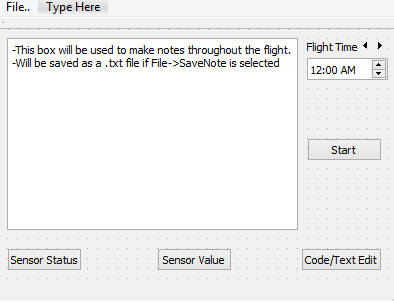
\includegraphics[width=\linewidth]{OLDGUI1.png}
	\label{Old GUI Home Page Layout}
\end{figure}
\begin{figure}